
%%%%%%%%%%%%%%%%%%%%%%% file typeinst.tex %%%%%%%%%%%%%%%%%%%%%%%%%
%
% This is the LaTeX source for the instructions to authors using
% the LaTeX document class 'llncs.cls' for contributions to
% the Lecture Notes in Computer Sciences series.
% http://www.springer.com/lncs       Springer Heidelberg 2006/05/04
%
% It may be used as a template for your own input - copy it
% to a new file with a new name and use it as the basis
% for your article.
% 
% NB: the document class 'llncs' has its own and detailed documentation, see
% ftp://ftp.springer.de/data/pubftp/pub/tex/latex/llncs/latex2e/llncsdoc.pdf
%
%%%%%%%%%%%%%%%%%%%%%%%%%%%%%%%%%%%%%%%%%%%%%%%%%%%%%%%%%%%%%%%%%%%
   

\documentclass{llncs}

\usepackage{amssymb}
\setcounter{tocdepth}{3}
\usepackage{graphicx}
 
% \usepackage{geometry}
% %\geometry{letterpaper}                   % ... or a4paper or a5paper or ...
% 
% \usepackage{xspace}
 
% \usepackage{epstopdf}
% \usepackage{graphicx,color}
% 
% 
\usepackage{booktabs}
\usepackage{datatool}
\usepackage{tikz}
\usepackage{pgfplots}
\usepackage{pgfplotstable}
\usetikzlibrary{patterns}
\usepackage{lscape}
\usepackage{subfig}

\usepackage{url}
\urldef{\mailsa}\path|{alfred.hofmann, ursula.barth, ingrid.haas, frank.holzwarth,|
\urldef{\mailsb}\path|anna.kramer, leonie.kunz, christine.reiss, nicole.sator,|
\urldef{\mailsc}\path|erika.siebert-cole, peter.strasser, lncs}@springer.com|    
\newcommand{\keywords}[1]{\par\addvspace\baselineskip
\noindent\keywordname\enspace\ignorespaces#1}

\begin{document}

\mainmatter  % start of an individual contribution

% first the title is needed
\title{Can Data Integration Quality be Enhanced on Multi-cloud using SLA?}

% a short form should be given in case it is too long for the running head
%\titlerunning{Lecture Notes in Computer Science: Authors' Instructions}

% the name(s) of the author(s) follow(s) next
%
% NB: Chinese authors should write their first names(s) in front of
% their surnames. This ensures that the names appear correctly in
% the running heads and the author index.
% 
\author{
 Daniel A. S. Carvalho\inst{1},
 Pl\'acido A. Souza Neto\inst{3},  
        Genoveva Vargas-Solar\inst{4},
          Nadia Bennani\inst{2},
        Chirine Ghedira\inst{1}       
}
%
\authorrunning{Lecture Notes in Computer Science: Authors' Instructions}
% (feature abused for this document to repeat the title also on left hand pages)

% the affiliations are given next; don't give your e-mail address
% unless you accept that it will be published
\institute{Universit\'e Jean Moulin, Lyon 3 MAGELLAN, IAE -- France \\
			\email{daniel.carvalho@univ-lyon3.fr, chirine.ghedira-guegan@univ-lyon3.fr}
		\and
		CNRS INSA-Lyon, LIRIS, UMR5205 -- France\\
			\email{nadia.bennani@insa-lyon.fr}
		\and
		Instituto Federal do Rio Grande do Norte, Natal -- Brazil \\
			\email{placido.neto@ifrn.edu.br}
		\and
		CNRS, LIG-LAFMIA, Saint Martin d'H\`eres -- France \\
			\email{genoveva.vargas@imag.fr}
		}

%
% NB: a more complex sample for affiliations and the mapping to the
% corresponding authors can be found in the file "llncs.dem"
% (search for the string "\mainmatter" where a contribution starts).
% "llncs.dem" accompanies the document class "llncs.cls".
%

\maketitle

 
% \begin{abstract}
% The abstract should summarize the contents of the paper and should
% contain at least 70 and at most 150 words. It should be written using the
% \emph{abstract} environment.
% 
% \keywords{We would like to encourage you to list your keywords within
% the abstract section}
% \end{abstract}


%\title{SLA-based Data Integration on Multi-Cloud: A Systematic Mapping Analysis}

\author{
        Daniel A. S. Carvalho\inst{1}, 
        Nadia Bennani\inst{2}, 
        Chirine Ghedira\inst{1}, 
        Pl\'acido A. Souza Neto\inst{3}, 
        Genoveva Vargas-Solar\inst{4}
 		}


\institute{
		Universit\'e Jean Moulin, Lyon 3 MAGELLAN, IAE -- France \\
			\email{danielboni@gmail.com, chirine.ghedira-guegan@univ-lyon3.fr}
		\and
		CNRS INSA-Lyon, LIRIS, UMR5205 -- France\\
			\email{nadia.bennani@insa-lyon.fr}
		\and
		Instituto Federal do Rio Grande do Norte, Natal -- Brazil \\
			\email{placido.neto@ifrn.edu.br}
		\and
		CNRS, LIG-LAFMIA, Saint Martin d'H\`eres -- France \\
			\email{genoveva.vargas@imag.fr}
		}
		
\maketitle

\begin{abstract}

\end{abstract}

\keywords{Systematic Mapping, Service Level Agreement, Data Integration, Multi-cloud Environment.}

% -------------------------------- Introduction -------------------------------- %
\section{Introduction}
\label{sec:intro}
The emergence of new architectures like the cloud opens new opportunities to data processing. 
The possibility of having unlimited access to cloud resources and the ``pay as U go'' model make it possible to change the hypothesis for processing big  data collections.  Instead of designing processes and algorithms taking into consideration  limitations on resources availability, the cloud sets the focus on the economic cost implied when using resources and producing results by parallelizing their use while delivering data under subscription oriented cost models.
 
Integrating and processing heterogeneous Big Data calls for efficient methods for correlating, associating, filtering them taking into consideration their ``structural'' characteristics (due to data variety) but also their quality (veracity), e.g., trust, freshness, provenance, partial or total consistency. 
Existing data integration techniques need to be revisited considering weakly curated and modeled data sets provided by different services under different quality conditions. Data integration can be done according to  (i) quality of service (QoS) requirements expressed by their consumers and (ii) Service Level Agreements (SLA)  exported by the cloud providers that host  Big Data and deliver resources for executing the associated management processes. Yet, it is not an easy task to completely enforce SLAs particularly because consumers use several cloud providers to store, integrate and process the data they require under the specific conditions they expect.
Naturally, a collaboration between cloud providers becomes necessary~\cite{036} but this should be also done in a user-friendly way, with some degree of transparency. 

To better understand, let us consider an example from the domain of energy
management. We assume we are interested in queries like: \textit{Give a list
of energy providers that can provision 1000 KW-h, in the next 10 seconds, that are close to my city, with a cost of 0,50 Euro/KW-h and that are labeled as green?} We consider a simplified SLA cloud contract inspired in the cheapest contract provided by Azure: \textit{cost of \$0,05 cents per call,  8~GB of I/O volume/month, free data transfer cost within the same region,  1~GB of storage.} 
Suppose that the user is ready to pay a maximum of \textit{\$5 as total query cost}; she requests that only  \textit{green} energy providers should be  listed (provenance), with at least  \textit{85$\%$} of precision of provided data, even if they are not fresh; she requires an availability rate of at least 90$\%$ and a response time of  \textit{0,01 s}. 
  The question is how can the user efficiently obtain  results for her queries such that they meet her QoS requirements, they respect her subscribed contracts with the involved cloud provider(s) and such that they do not neglect services contracts? 
  %Particularly, for queries that call several services deployed  on different clouds.

%\subsection{Contribution}
Data integration has to be revisited according to  the properties of data collections (volume, variety, velocity), to service oriented data provision contexts normally done in the context of cloud environments. Such environments (multi-cloud)  provide the required storage, computing and processing resources but they call for new strategies for integrating data considering different SLAs, subscription conditions, and data consumption requirements and preferences. In this context, the contribution of our work is two-fold. First it proposes a classification scheme of existing works fully or partially addressing the problem of integrating data in multi-cloud environments eventually taking into consideration Service Level Agreement. Second, the description of our vision  for guiding data integration in multi-cloud environments  by SLA and user/applications preferences. 

The classification scheme results from  applying the  methodology defined in~\cite{SM:Petersen:2008} called  \textit{systematic mapping}  for defining a classification of a field. A classification consists of categories clustered into facets in which publications (i.e., papers) are aggregated according to frequencies (i.e., number of published papers). According to the methodology, the study consists in  five interdependent tasks including (i) the definition of a research scope by defining research questions; (ii) retrieving candidate papers by querying different scientific databases (e.g. IEEE, Citeseer, DBLP); (iii) selecting relevant papers that can be used for answering the research questions by defining inclusion and exclusion criteria; (iv) defining a classification scheme by analyzing the abstracts of the selected papers to identify the terms that will be used as categories for classifying the papers; (v) producing a systematic mapping by sorting papers according to the classification scheme. 

Our final objective by applying the systematic mapping methodology is to identify trends and open issues regarding data integration in multi-cloud environments. Thus, our classification scheme consists in four facets that classify existing scientific publications addressing  together or independently SLA, Data Integration in Multi-cloud environments. We define two additional facets to identify the type of papers (e.g., position, survey, etc) and the type of contribution (e.g., model, architecture, system). It shows the research trends of data integration as a result of the emergence of the cloud and the characteristics associated to Big Data processing. The study and the classification scheme that we propose support  the proposal of our vision for filling some gaps and propose an original data integration solution according to current trends in the area. 


%\subsection{Organization of the paper}
The remainder of this paper is organized as follows. 
Section~\ref{sec:sm} describes our study of  data integration perspectives and the evolution of the research works that address some aspects of the problem. The section gives a quantitative analysis of our study and identifies open issues in the field. Section \ref{sec:approach} gives the general lines of the approach we propose for guiding data integration using SLA agreements in a multi-cloud environment.  Section~\ref{sec:rw} discusses existing approaches studying data integration problems in multi-cloud contexts that take into account SLA contacts.
Section~\ref{sec:conc} concludes the paper and discusses future work. 


 
% --------------------------------              -------------------------------- %
 
%. . . . . . . . . . . . . . . . . . . . . . . . . . . . . . . . . . . . . . . . . . . . . . . . . . . . . . . . . . . . . . . . . . . . . . . . . . . . . . . . . . . . 
\section{Data integration challenges: classification scheme}\label{sec:sm}
%. . . . . . . . . . . . . . . . . . . . . . . . . . . . . . . . . . . . . . . . . . . . . . . . . . . . . . . . . . . . . . . . . . . . . . . . . . . . . . . . . . . . 
\section{Systematic mapping process}\label{sec:sm}

\iplacido{I changed the word expression `step' to `task' in order to describe
the methodology `workflow'.}  
%We applied the systematic mapping methodology presented
% in~\cite{SM:Petersen:2008} to our study on SLA-guided data integration on a multi-cloud environments.
The methodology defined in~\cite{SM:Petersen:2008} presents some guidelines to
performing a systematic mapping review in software engineering research
context. The systematic mapping is a defined method to build
a classification of a field of interest. The results analysis focuses on
frequencies of publications for categories (facets).  

The process workflow describes five interdependent tasks: \textit{(i)}
\textbf{definition of research question} to define the \textit{research scope}; \textit{(ii)} textbf{conduct search} in
order to retrieve \textit{all candidate papers}. Those papers are selected applying a query which
express the research interest to scientific databases; \textit{(iii)}
\textbf{screening of papers} to select the \textit{relevant papers} to answer the research
question based on a inclusion and exclusion criteria; \textit{(iv)}
\textbf{keywording using abstracts} to identify terms that helps on developing the
\textit{classification scheme} (mapping categories to classify the papers); and
\textit{(v)} \textbf{fata extraction and mapping process} to sort the relevant
papers into the mapping categories and produce the systematic mapping.

 
% \begin{description}
% \item \textbf{Definition of research question} to define the \textit{research scope};
% \item \textbf{Conduct search} in order to retrieve \textit{all candidate papers}. Those papers are selected applying a query which express the research interest to scientific databases;
% \item  \textbf{Screening of papers} to select the \textit{relevant papers} to answer the research question based on a inclusion and exclusion criteria;
% \item \textbf{Keywording using abstracts} to identify terms that helps on developing the \textit{classification scheme} (mapping categories to classify the papers); and
% \item \textbf{Data extraction and mapping process} to sort the relevant papers into the mapping categories and produce the systematic mapping.
% \end{description}

% The following subsections describes our first to fourth step in the
% mapping. %The systematic mapping results are presented in the next section.   
 
  
\iplacido{Defining references to the RQs.} 
\subsection{Research questions (RQs)}
The aim of this work is to identify in the literature how has \textit{SLA-guided
data integration on a multi-cloud environments} been explored, discover possible
gaps and the main results produced.    
In order to achieve this goal we formulated three research questions:
\begin{enumerate}
\item \textbf{RQ1:} Which are the SLA measures that have been applied most in
the cloud?
\item \textbf{RQ2:}  How has the publication of papers on data integration
involved towards cloud topics?
\item \textbf{RQ3:} How and in which context have data integration guided by QoS
models or requirements been explored in the literature?
\end{enumerate}

\subsection{Search and screening of papers} \label{subsec:search}

Based on the research questions and our research interests, a set of keywords were defined in order to 
retrieve relevant papers.
As mentioned before, we are interested in merging three different topics: SLA, Data Integration and Multi-cloud.
According to these keywords and correlated words the search query formulated was:
\medskip  \\
%\begin{small}
%\begin{verbatim}
%(("SLA" OR "Service Level Agreement" OR "Service-Level Agreement") AND 
%   ("Cloud" OR "Multi-cloud" OR "Multi cloud" OR "Multicloud" OR "Inter-cloud" OR 
%      "Inter cloud" OR "Intercloud" OR "Federated cloud" OR "Cloud federation" OR 
%         "Hybrid cloud")) OR
%(("SLA" OR "Service Level Agreement" OR "Service-Level Agreement") AND 
%   ("Data Integration" OR "Data Integration Systems" OR "Sources Integration" OR 
%      "Multi Databases" OR "Multi-databases" OR "Multidatabases" OR 
%         "Distributed databases")) OR
%(("Data Integration" OR "Data Integration Systems" OR "Sources Integration" OR 
%   "Multi Databases" OR "Multi-databases" OR "Multidatabases" OR 
%      "Distributed databases") AND 
%   ("Cloud" OR "Multi-cloud" OR "Multi cloud" OR "Multicloud" OR "Inter-cloud" OR 
%      "Inter cloud" OR "Intercloud" OR "Federated cloud" OR "Cloud federation" OR 
%        "Hybrid cloud")) OR
%(("Data Integration" OR "Data Integration Systems" OR "Sources Integration" OR 
%   "Multi Databases" OR "Multi-databases" OR "Multidatabases" OR 
%      "Distributed databases") AND 
%   ("QoS" and "Quality of Service"))
%\end{verbatim}
%\end{small}
\daniel{New format of the query. We saved some space.}
\begin{small}
\textit{(("SLA" OR "Service Level Agreement" OR "Service-Level Agreement") AND 
   ("Cloud" OR "Multi-cloud" OR "Multi cloud" OR "Multicloud" OR "Inter-cloud" OR 
      "Inter cloud" OR "Intercloud" OR "Federated cloud" OR "Cloud federation" OR 
\medskip        "Hybrid cloud"))} \textbf{OR} \\ 
\textit{(("SLA" OR "Service Level Agreement" OR "Service-Level Agreement") AND 
   ("Data Integration" OR "Data Integration Systems" OR "Sources Integration" OR 
      "Multi Databases" OR "Multi-databases" OR "Multidatabases" OR }
\medskip        \textit{ "Distributed databases"))} \textbf{OR} \\
\textit{(("Data Integration" OR "Data Integration Systems" OR "Sources Integration" OR 
   "Multi Databases" OR "Multi-databases" OR "Multidatabases" OR 
      "Distributed databases") AND 
   ("Cloud" OR "Multi-cloud" OR "Multi cloud" OR "Multicloud" OR "Inter-cloud" OR 
      "Inter cloud" OR "Intercloud" OR "Federated cloud" OR "Cloud federation" OR }
\medskip       \textit{ "Hybrid cloud"))} \textbf{OR} \\
\textit{(("Data Integration" OR "Data Integration Systems" OR "Sources Integration" OR 
   "Multi Databases" OR "Multi-databases" OR "Multidatabases" OR 
      "Distributed databases") AND 
   ("QoS" and "Quality of Service"))}
\end{small}
\medskip

We searched and filtered relevant works in four steps.
In the first step we searched in four scientific databases: IEEE~\footnote{http://ieeexplore.ieee.org/},
ACM~\footnote{http://dl.acm.org/}, Science Direct~\footnote{http://www.sciencedirect.com/} and
CiteSeerX~\footnote{http://citeseerx.ist.psu.edu/}.
We retrieved 1832 publications (See table~\ref{table:pub}).

\begin{table}[!htb]
\begin{center}
\begin{tabular}{>{\centering\arraybackslash}p{2.5cm}|>{\centering\arraybackslash}p{2.5cm}|>{\centering\arraybackslash}p{2.5cm}|>{\centering\arraybackslash}p{2.5cm}}
\toprule
\textbf{Database} & \textbf{Amount} & \textbf{Included} & \textbf{Excluded} \\ 
\hline \toprule
\textbf{IEEE} & 658 & 56 & 602 \\ 
\hline 
\textbf{AMC} & 649 & 31 & 618	 \\ 
\hline 
\textbf{Science Direct} & 106 & 6 & 100 \\ 
\hline 
\textbf{CiteSeerX} & 419 & 21 & 398 \\ 
\hline 
\textit{Total} & 1832 & \textbf{114} & 1718 \\ 
\bottomrule \hline
\end{tabular} 
\end{center}
\caption{Sources and number of papers}\label{table:pub}
\end{table}

%In the second step, we added all papers into \textit{Mendeley}~\footnote{http://www.mendeley.com/} 
%reference manager.
%Using Mendeley's plugin an bibtex file containing all papers was exported. 
%This file was used to create a spreadsheet summarizing all papers retrieved, including their abstracts,
%source, year and authors. 

\daniel{Why did we choose this criteria.}
We performed the filtering procedure by analyzing the title and the abstract of the papers in the
third step. 
Based on our inclusion and exclusion criteria described in the table~\ref{table:criteria}, we looked for 
papers that are relevant to our study. 
This criteria was defined taking into account our research interests. 
We are looking for works regarding data integration on a multi-cloud environment using SLA.
In this process 1718 publications were excluded. 
The columns \textbf{Included} and \textbf{Excluded} in table~\ref{table:criteria} summarize the number of papers that were considered to each source on our mapping.

\begin{table}[!htb]
\begin{center}
\begin{tabular}{p{10cm}}
\bottomrule \hline
\textbf{Inclusion criteria} \\ 
\hline 
- The text must be in English \\ 
- SLA approaches including data integration and/or multi-cloud environments\\
- Studies regarding SLA and cloud, describing models, languages and security issues \\
- Works describing improvements to SLA \\
- Data integration studies including cloud and/or multi-cloud  \\
- Quality of Service efforts regarding data integration \\
\bottomrule \hline 
\textbf{Exclusion criteria} \\ 
\hline 
- Publication with only power point version available \\ 
- SLA approaches regarding resource allocation \\
- Publications outside of the software engineering area \\
- Any paper out of the inclusion criteria  \\
\bottomrule \hline
\end{tabular} 
\end{center}
\caption{Inclusion and exclusion criteria}\label{table:criteria}
\end{table}

Finally, in the fourth step, we built the final data collection composed by 114 publications.

\subsection{Keywording of abstracts}

\idaniel{Why did we choose our facets and dimensions.}
Considering the criterias discussed previously (subsection~\ref{subsec:search}),
114 works were selected to our study. 
According to our research interests, these papers were classified into the five facets. 
The facets' dimensions were defined based on our knowledge and on the keywording process proposed by the
methodology.   
For each paper, the abstract
was analyzed in order to identify the contribution for each facet.
As result to this process, each paper is classified into the dimensions of each facet. 
The results are summarized in tables \ref{table:dienviron} to \ref{table:contribution}. 
The five facets are described bellow.

\textbf{Data Integration Environment facet} (See table~\ref{table:dimensions}). 
Represents the environment (architecture and deployment) in which data integration is being applied.
The dimensions to this facet are: Cloud, Data Warehouse, Federated Database and Multi-cloud.
%\begin{table}[h]
%\begin{center}
%\begin{tabular}{p{4cm}p{10cm}}
%\hline 
%\textbf{Dimension} & \textbf{Publication} \\ 
%\hline 
%Cloud & 
%\cite{106,110,105,107,108,109,068,070,072,113,073,074,075,076,077,078,079,081,082,083,085,087,088,089,090,094,095,096,097,098,099,100,102,103}\\ 
%\hline 
%Data Warehouse & \cite{066,114,091} \\ 
%\hline 
%Federated Database & \cite{071,089,112} \\ 
%\hline 
%Multi-cloud & \cite{012,071,093} \\ 
%\hline 
%\end{tabular}
%\end{center}
%\caption{Data Integration Environment facet}\label{table:dienviron}
%\end{table}

\textbf{Data Integration Description facet} (See table~\ref{table:dimensions}).
Indicates the strategy used by authors in order to achieve data integration. 
The dimensions to this facet are: Knowledge, Metadata and Schema.
%\begin{table}[h]
%\begin{center}
%\begin{tabular}{p{4cm}p{10cm}}
%\hline 
%\textbf{Dimension} & \textbf{Publication} \\ 
%\hline 
%Knowledge & \cite{012,083} \\ 
%\hline 
%Metadata & \cite{108,066,113} \\ 
%\hline 
%Schema & \cite{070,071,072,073,075,114,083,089,091,112,102} \\ 
%\hline 
%\end{tabular}
%\end{center}
%\caption{Data Integration Description facet}\label{table:didesc}
%\end{table}

\textbf{Data Quality facet} (See table~\ref{table:dimensions}). 
Refers to data quality parameters applied in the publication. 
The dimensions are: Confidentiality, Privacy, Security, SLA, Data Protection, Data Provenance and Others.
Note that a publication is classified in the SLA dimension when it does not focus on a specific quality parameter, but in general uses a SLA contract in order to specify one or more.
%\begin{table}[h]
%\begin{center}
%\begin{tabular}{p{4cm}p{10cm}}
%\hline 
%\textbf{Dimension} & \textbf{Publication} \\ 
%\hline 
%Confidentiality & \cite{104,109,111,024} \\ 
%\hline 
%Privacy & \cite{109,111,007,067,068,113,024,047,095,096} \\ 
%\hline 
%Security & \cite{109,113,081,093,112,065} \\ 
%\hline 
%SLA  &\cite{044,001,002,007,008,009,011,012,013,014,015,016,017,018,019,046,020,021,022,024,025,026,027,028,029,030,031,032,035,034,036,037,038,039,040,041,042,023,043,045,047,048,049,050,051,052,053,054,055,056,057,058,060,059,061,062,063,064,065,033}\\
%\hline 
%Data Protection & \cite{106,104,047} \\ 
%\hline 
%Data Provenance & \cite{012} \\ 
%\hline 
%Others & \cite{071,093,100} \\ 
%\hline 
%\end{tabular}
%\end{center}
%\caption{Data Quality facet}\label{table:dq}
%\end{table}

\textbf{SLA facet} (See table~\ref{table:dimensions}).
This facet is devote to present how the SLA is mainly used in the publication. 
The dimension for this facet are: Language, Model, Resources and Security.
It is important to see that SLA appears as a dimension and as a facet.
As a facet, we are interest in the way SLA is used. 
As a dimension, it is just to indicate that the work
applies SLA in your solution.
%\begin{table}[h]
%\begin{center}
%\begin{tabular}{p{4cm}p{10cm}}
%\hline 
%\textbf{Dimension} & \textbf{Publication} \\ 
%\hline 
%Language & \cite{003,037,039,041,055,056,061} \\ 
%\hline 
%Model & \cite{044,001,002,005,003,006,007,008,009,010,012,013,014,015,016,017,018,019,046,020,021,022,024,026,027,028,029,030,031,032,035,036,038,040,042,023,043,045,047,048,049,050,051,053,054,055,057,058,060,059,061,063,033}\\ 
%\hline 
%Resources & \cite{110,053,064} \\ 
%\hline 
%Security & \cite{109,011,113,025,035,034,081,038,049,050,052,093,062,112,065} \\ 
%\hline 
%\end{tabular}
%\end{center}
%\caption{SLA facet}\label{table:sla}
%\end{table}

\textbf{Contribution facet} (See table~\ref{table:dimensions}).
Express the kind of contribution proposed by the author. 
The dimensions are Tool, Literature Analysis, Method, Model, Process and Extended Study.
%\begin{table}[h]
%\begin{center}
%\begin{tabular}{p{4cm}p{10cm}}
%\hline 
%\textbf{Dimension} & \textbf{Publication} \\ 
%\hline 
%Tool & \cite{110,001,002,005,066,068,070,071,011,014,015,016,019,046,113,024,074,077,026,078,028,029,032,035,081,086,087,088,053,054,091,056,093,094,095,061,112,064,065}\\ 
%\hline 
%Literature Analysis & \cite{105,108,109,111,004,003,069,010,073,038,042,089,048,052,099,103} \\ 
%\hline 
%Method & \cite{106,107,011,075,076,043,051,092,101,102} \\ 
%\hline 
%Model & \cite{044,006,007,066,067,008,009,070,012,071,072,013,017,018,020,114,027,079,030,031,034,036,080,082,037,083,084,039,040,085,041,087,088,045,090,049,050,055,056,057,058,060,059,096,062,098,063,033}\\  
%\hline 
%Process & \cite{021,022,025,023,096,100} \\ 
%\hline 
%Extended Study & \cite{104,047,097} \\ 
%\hline 
%\end{tabular}
%\end{center}
%\caption{Contribution facet}\label{table:contribution}
%\end{table}

\textbf{Research facet} (See table~\ref{table:dimensions}).
Dedicates to classify in which kind of research the publication can be fitted in. 
The dimensions to this facet are: Evaluation research, Validation research, Solution proposal 
and Opinion papers.

%\begin{table}[h]
%\begin{center}
%\begin{tabular}{p{4cm}p{10cm}}
%\hline 
%\textbf{Dimension} & \textbf{Publication} \\ 
%\hline 
%Evaluation research & \cite{008,026,048,069,073,074,089,094,099,102,103,105,111} \\ 
%\hline 
%Validation research & \cite{001,002,005,006,007,009,011,012,014,015,016,017,018,019,020,021,022,023,024,025,027,028,029,030,031,032,033,034,036,037,039,045,051,057,059,079,095,098,100,105,112}\\
%\hline 
%Solution proposal & \cite{008,035,038,040,041,042,043,044,046,047,048,049,050,051,053,054,055,056,058,060,061,062,063,064,065,066,067,068,070,071,072,075,076,077,078,079,080,081,082,083,084,085,086,087,088,090,091,092,093,094,095,096,097,098,100,101,102,104,106,107,110,113,114}\\
%\hline 
%Opinion paper & \cite{003,004,010,013,052,069,073,108,109} \\ 
%\hline  
%\end{tabular}
%\end{center}
%\caption{Research facet}\label{table:research}
%\end{table}

\idaniel{New table...}
\begin{table}[!h]
\begin{center}
\begin{tabular}{p{4cm}p{10cm}}
\hline 
\textbf{Dimension} & \textbf{Publication} \\ 
\hline 
Cloud & 
\cite{106,110,105,107,108,109,068,070,072,113,073,074,075,076,077,078,079,081,082,083,085,087,088,089,090,094,095,096,097,098,099,100,102,103}\\ 
\hline 
Data Warehouse & \cite{066,114,091} \\ 
\hline 
Federated Database & \cite{071,089,112} \\ 
\hline 
Multi-cloud & \cite{012,071,093} \\ 
\hline 
Knowledge & \cite{012,083} \\ 
\hline 
Metadata & \cite{108,066,113} \\ 
\hline 
Schema & \cite{070,071,072,073,075,114,083,089,091,112,102} \\ 
\hline 
Confidentiality & \cite{104,109,111,024} \\ 
\hline 
Privacy & \cite{109,111,007,067,068,113,024,047,095,096} \\ 
\hline 
Security & \cite{109,113,081,093,112,065} \\ 
\hline 
SLA  &\cite{044,001,002,007,008,009,011,012,013,014,015,016,017,018,019,046,020,021,022,024,025,026,027,028,029,030,031,032,035,034,036,037,038,039,040,041,042,023,043,045,047,048,049,050,051,052,053,054,055,056,057,058,060,059,061,062,063,064,065,033}\\
\hline 
Data Protection & \cite{106,104,047} \\ 
\hline 
Data Provenance & \cite{012} \\ 
\hline 
Others & \cite{071,093,100} \\ 
\hline 
Language & \cite{003,037,039,041,055,056,061} \\ 
\hline 
Model & \cite{044,001,002,005,003,006,007,008,009,010,012,013,014,015,016,017,018,019,046,020,021,022,024,026,027,028,029,030,031,032,035,036,038,040,042,023,043,045,047,048,049,050,051,053,054,055,057,058,060,059,061,063,033}\\ 
\hline 
Resources & \cite{110,053,064} \\ 
\hline 
Security & \cite{109,011,113,025,035,034,081,038,049,050,052,093,062,112,065} \\ 
\hline 
Tool & \cite{110,001,002,005,066,068,070,071,011,014,015,016,019,046,113,024,074,077,026,078,028,029,032,035,081,086,087,088,053,054,091,056,093,094,095,061,112,064,065}\\ 
\hline 
Literature Analysis & \cite{105,108,109,111,004,003,069,010,073,038,042,089,048,052,099,103} \\ 
\hline 
Method & \cite{106,107,011,075,076,043,051,092,101,102} \\ 
\hline 
Model & \cite{044,006,007,066,067,008,009,070,012,071,072,013,017,018,020,114,027,079,030,031,034,036,080,082,037,083,084,039,040,085,041,087,088,045,090,049,050,055,056,057,058,060,059,096,062,098,063,033}\\  
\hline 
Process & \cite{021,022,025,023,096,100} \\ 
\hline 
Extended Study & \cite{104,047,097} \\ 
\hline 
Evaluation research & \cite{008,026,048,069,073,074,089,094,099,102,103,105,111} \\ 
\hline 
Validation research & \cite{001,002,005,006,007,009,011,012,014,015,016,017,018,019,020,021,022,023,024,025,027,028,029,030,031,032,033,034,036,037,039,045,051,057,059,079,095,098,100,105,112}\\
\hline 
Solution proposal & \cite{008,035,038,040,041,042,043,044,046,047,048,049,050,051,053,054,055,056,058,060,061,062,063,064,065,066,067,068,070,071,072,075,076,077,078,079,080,081,082,083,084,085,086,087,088,090,091,092,093,094,095,096,097,098,100,101,102,104,106,107,110,113,114}\\
\hline 
Opinion paper & \cite{003,004,010,013,052,069,073,108,109} \\ 
\hline  
\end{tabular}
\end{center}
\caption{List of publications per dimension}\label{table:dimensions}
\end{table}


 % Mapping Process %
% --------------------------------              -------------------------------- %

%\section{Quantitative Analysis}\label{sec:qanalysis}

This section shows the analysis and discussion of our Systematic Mapping results.
We proceed by presenting bubble charts as result of combining different facets in order to 
\textit{(i)} answer the research questions and \textit{(ii)} to justify our proposal.


\subsection{Combining the facets Contribution, SLA and Data Integration Description}

\begin{figure}[h!]
\centering
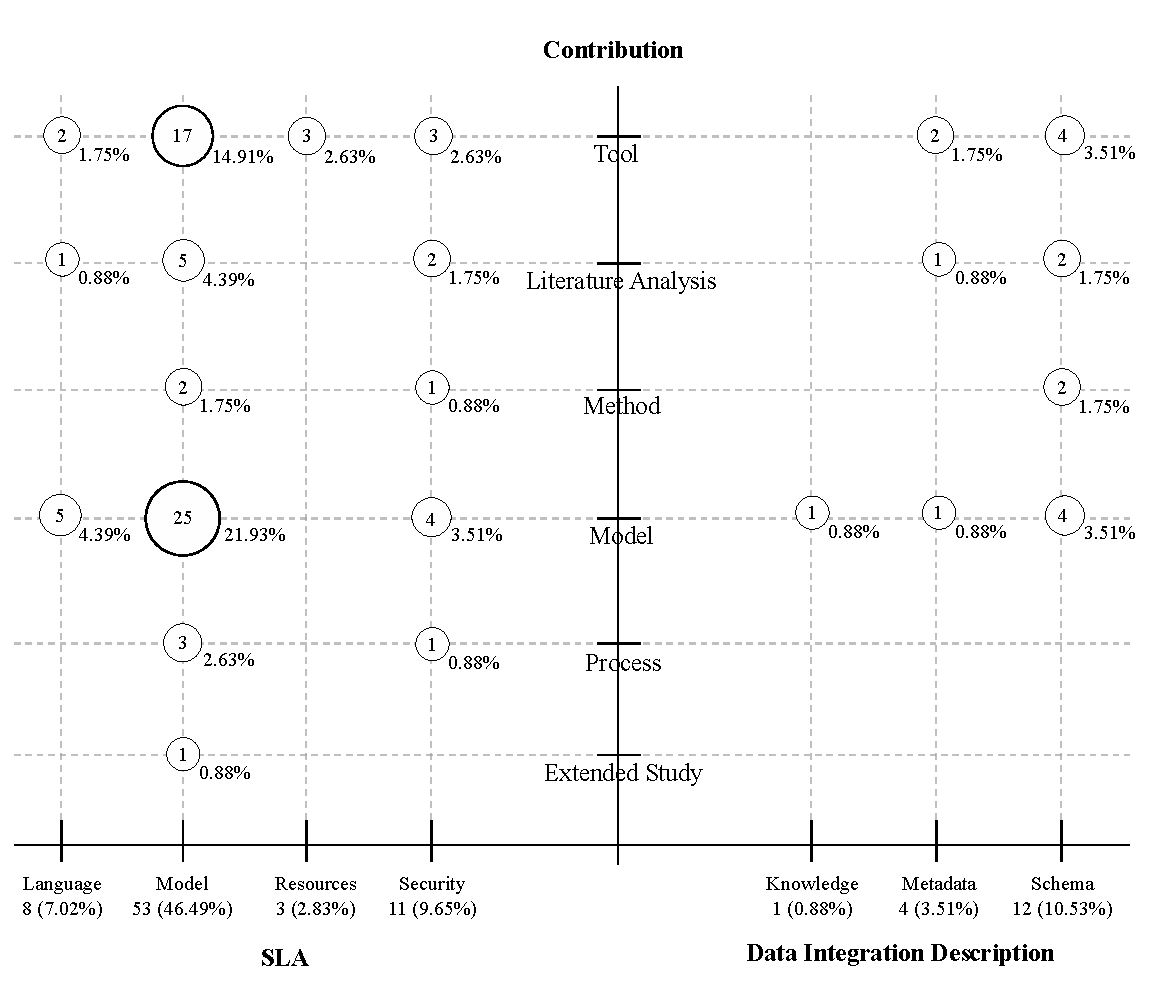
\includegraphics[scale=0.56]{figs/bubble-charts/Contribution-SLA-DIdescription.pdf} 
\caption{Contribution, SLA and Data Integration Description}\label{fig:facet1}
\end{figure}

Combining the facet contribution with the facets SLA and data integration description 
(Figure~\ref{fig:facet1}) it is possible to obtain two analysis: 
(i) how the SLA has been applied to scientific works and which are the type of contribution 
most proposed by the authors; and (ii) which are the most applied data integration description
strategy in papers and which are the most type of contribution associated to these works. 
Looking to the figure you can note that models for SLA have been the focus in the papers 
(53 appearances - 46.49\%) followed by Security (11 appearances - 9.65\%), Language 
(8 appearances - 7.02\%) and Resources (3 appearances - 22.83\%).
Analyzing the figure is also possible to observe that Model (34 appearances - 29.82\%) and 
Tool (25 appearances - 21.93\%) are the mainly type of contribution proposed in the papers 
followed by Literature Analysis (8 appearances - 7.02\%), Process (4 appearances - 3.51\%), 
Method (3 appearances - 2.63\%) and Extended Study (1 appearance - 0.88\%).
Regarding the data integration description, Schema (12 appearances - 10.53\%) is the most 
applied dimension followed by Metadata (4 appearances - 3.51\%) and Knowledge (1 appearance - 0.88\%).

\subsection{Combining the facets Data Integration Environment, Contribution and Research}

\begin{figure}[h]
\centering
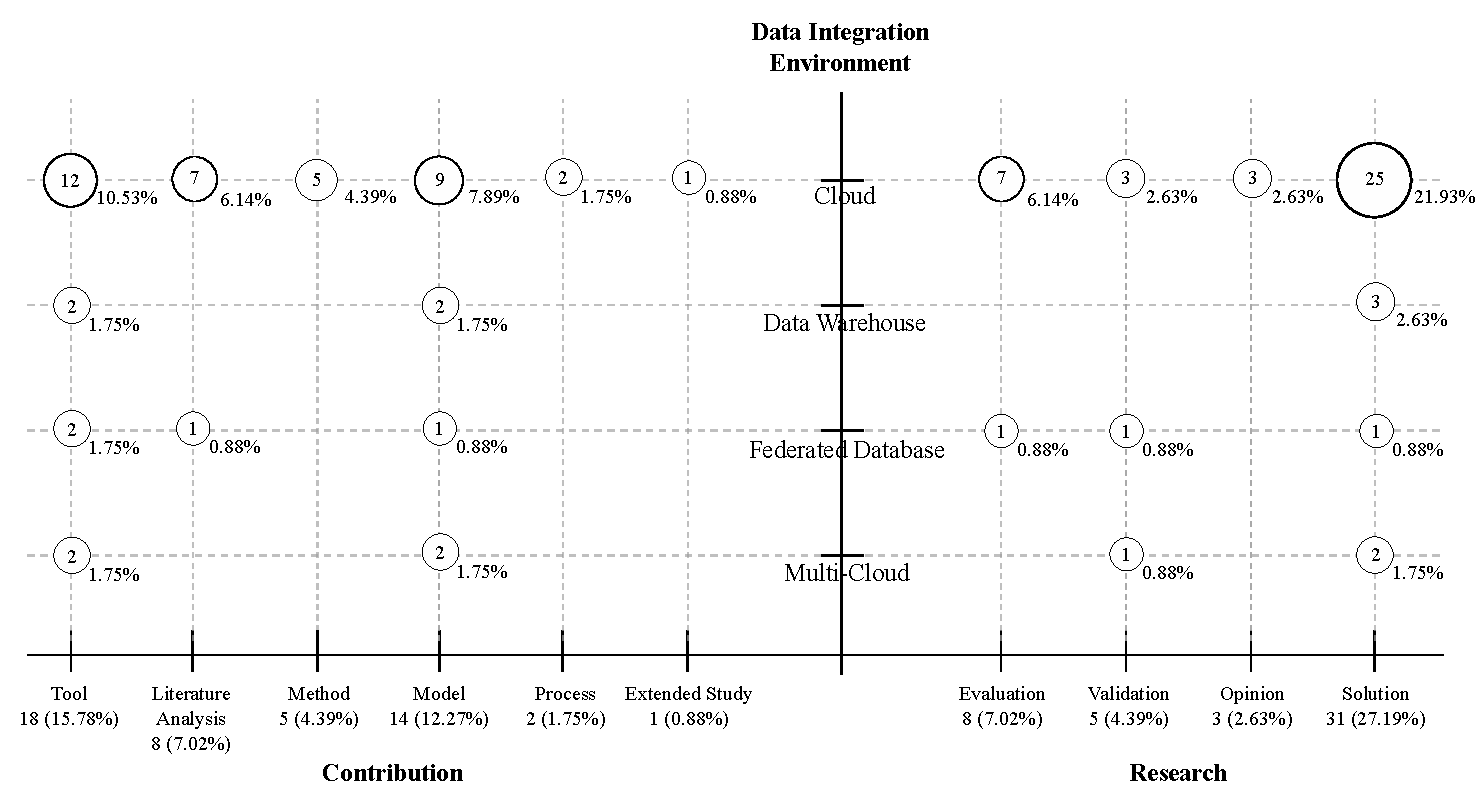
\includegraphics[scale=0.48]{figs/bubble-charts/DI-Environment-Contribution-Research.pdf}
\caption{facets Data Integration Environment, Contribution and Research}\label{fig:facet2}
\end{figure}

Combining the facet data integration environment with the facets contribution and research 
(Figure~\ref{fig:facet2}) it is possible to observe which are the most proposed type of
contribution and research applied to the different data integration environments.  
Looking to the figure it is possible to identify that Tool (18 appearances - 15.78\%) and 
Model (14 appearance - 12.27\%) are the mainly type of contribution developed, 
followed by Literature Analysis (8 appearances - 7.02\%), Method (5 appearances - 4.39\%) 
Process (2 appearances - 1.75\%) and Extended Study (1 appearance - 0.88\%).
Analyzing the figure is also possible to observe that Solution (31 appearances - 27.19\%) is 
the type of research most proposed, 
followed by Evaluation (8 appearances - 7.02\%), Validation (5 appearances - 4.39\%) and
Opinion (3 appearances - 2.63\%).

\iplacido{`Old' figure 3 deleted\ldots} 
 
% \subsection{Combining the facets SLA and Contribution}
% 
% Combining the facet SLA with the facet contribution (Figure~\ref{fig:facet3}) it is possible 
% to observe how the SLA has been applied to scientific works and which are the type of contribution 
% most proposed by the authors.
% Looking to the figure you can remark that models for SLA have been the focus of the most papers 
% (53 appearances).
% Analyzing the figure is also possible to observe that Model (34 appearances - 29.82\%) and 
% Tool (25 appearances - 21.93\%) are the mainly type of contribution proposed in the papers 
% followed by Literature Analysis (8 appearances - 7.02\%), Process (4 appearances - 3.51\%), 
% Method (3 appearances - 2.63\%) and Extended Study (1 appearance - 0.88\%).
% 
% \begin{figure}[h!]
% \centering
% 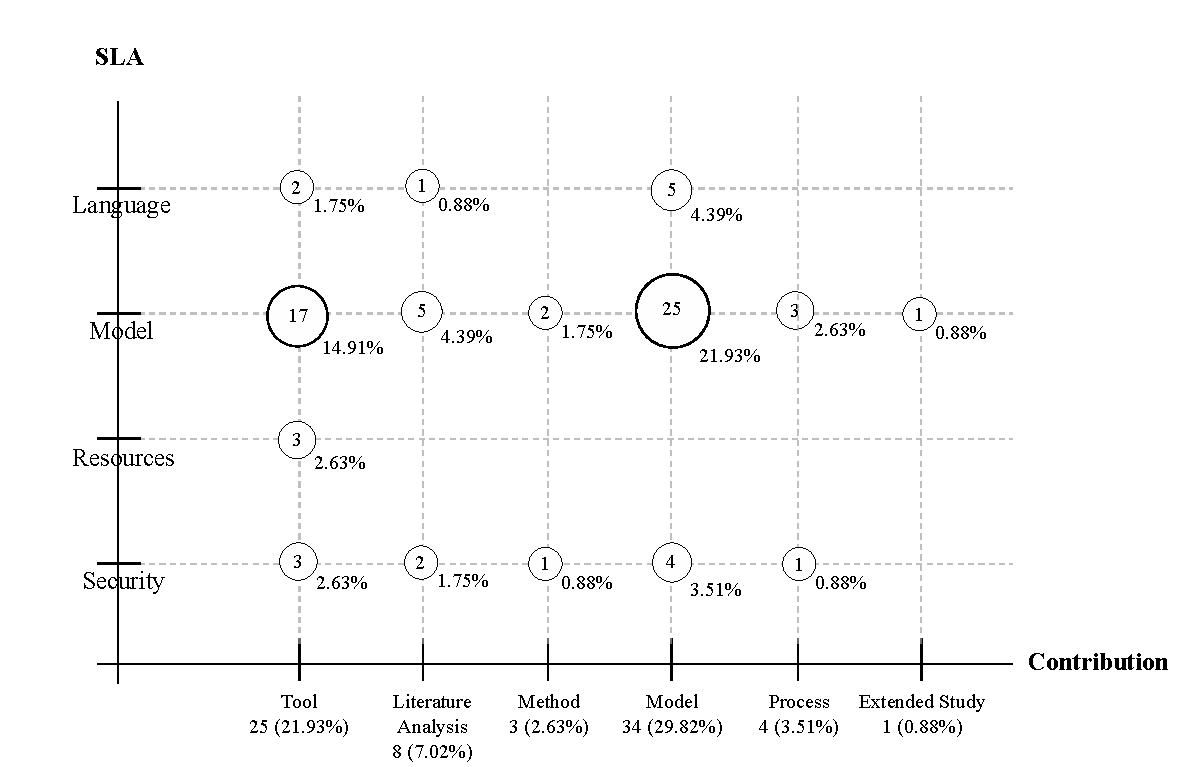
\includegraphics[scale=0.65]{figs/bubble-charts/SLA-Contribution.pdf}
% \caption{Facets SLA and Contribution}\label{fig:facet3}
% \end{figure}


\subsection{Combining the facets Data Quality, Data Integration Environment and Data Integration Description}

Combining the facet data quality with the facets data integration environment and data integration description
(Figure~\ref{fig:facet4}) it is possible to note which quality of service parameters have been applied most in
data integration studies.
It is also possible to identify which are the most applied data integration environment and description.
First of all, security and privacy are the most applied QoS parameter (5 appearance - 4.39\%)
followed by the other dimensions (1 appearance - 0.88\%). 
The figure also shows that SLA has not been widely used in order to address data integration solutions
(1 appearance) which reinforces our main objective of integrate SLA, data integration and multi-cloud 
environments. 
Analyzing the figure is also possible to observe that the most deployed data integration environment is 
the cloud (9.68\%) followed by multi-cloud (4.39\%), federated databases (1.75\%) and data warehouse (0.00\%).
The data integration description dimensions had the same percentage for schema, knowledge and metadata (2 appearance - 1.75\%)

\begin{figure}[!h]
\centering
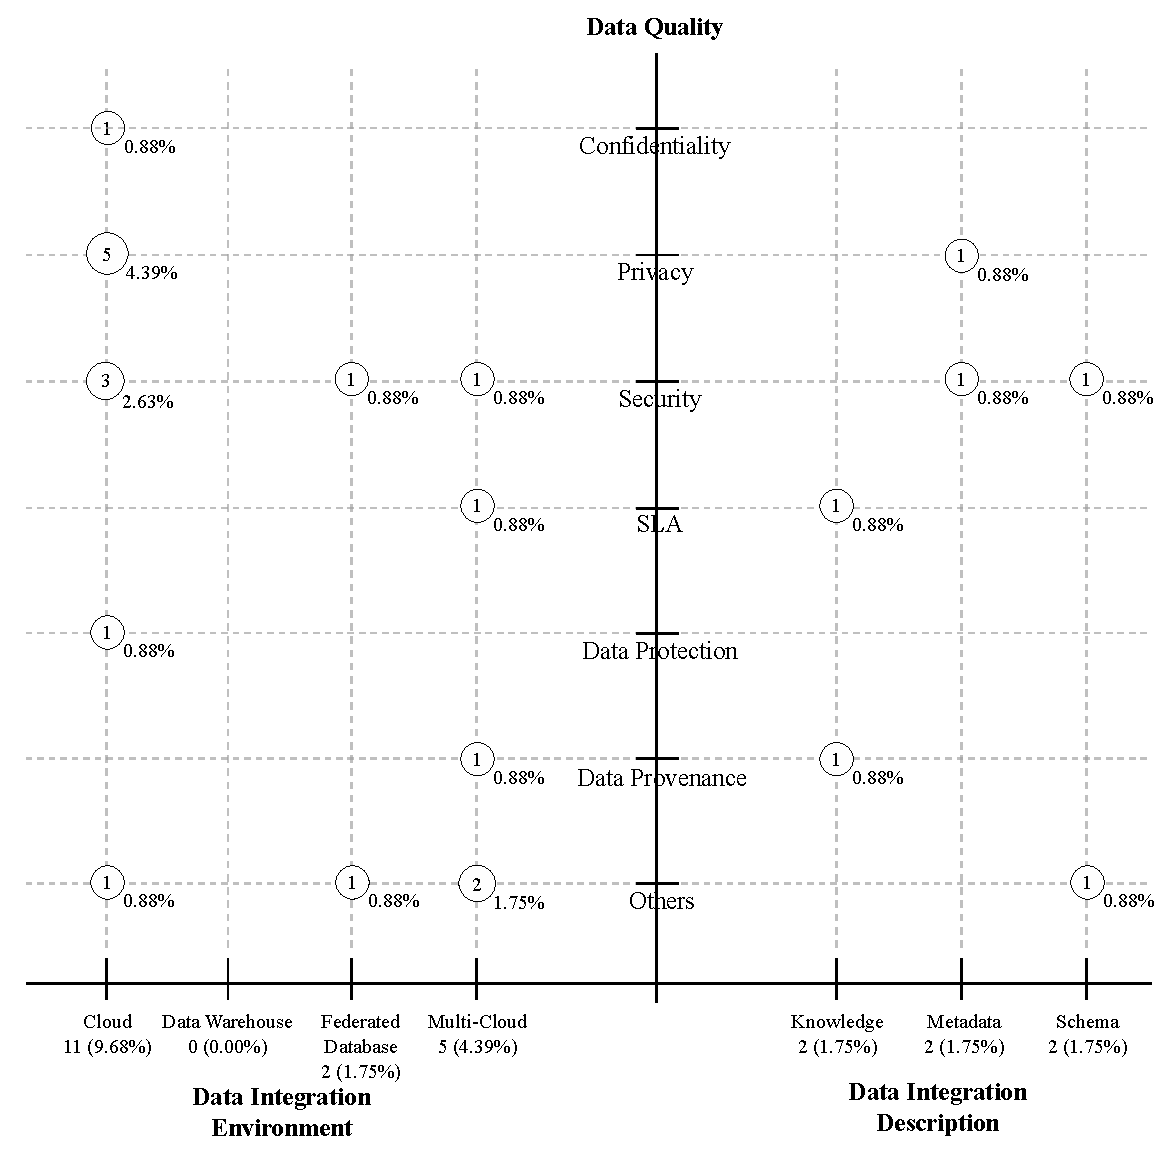
\includegraphics[scale=0.53]{figs/bubble-charts/Data-Quality-DI.pdf}
\caption{Facets Data Quality, Data Integration Environment and Data Integration Description}\label{fig:facet4}
\end{figure}
 % Quantitative Analysis %
% --------------------------------              -------------------------------- %

%-[BEGIN]-----------------------------------------------------------------------
%\section{Enhancing  Data Integration on Multi-Cloud environments with SLA}\label{sec:approach}
%-[END]-----------------------------------------------------------------------
%This paper introduces the challenge of integrating data from distributed data services deployed on different cloud providers guided by service level agreements (SLA) and user preferences statements. The data integration problem is stated as a continuos data provision problem that has an associated economic cost and that uses automatic learning techniques for ensuring different qualities of delivered data (fresh, precise, partial).
Current big data settings impose to consider SLA and different data delivery models. We believe that given the volume and the complexity of query evaluation that includes steps that imply greedy computations, it is important to combine and revisit well-known solutions adapted to these contexts. We are currently developing the strategies and algorithms sketched here applied to energy consumption applications as the one described in the paper and also to elections and political campaign data integration in order to guide decision making on campaign strategies. % Approach ... %

% -------------------------------- Related Works ------------------------------- %
%\section{Related Works}\label{sec:rw}
%%-[BEGIN]-----------------------------------------------------------------------
\section{Related Works}\label{sec:rw}
%This section contains the background necessary to develop the research.
Regarding our problem, two different lines of research were targeted:
\textit{(i)} data integration on a multi-cloud environment; and
\textit{(ii)} service level agreements and data integration.
%There are two different lines of research interesting to the proposal:

\subsection{Data integration on multi-cloud environment}
Correndo \textit{et al}~\cite{075} proposed an method for achieving RDF data integration
using SPARQL query rewrinting. 
The proposal takes into account other already existent approaches regarding rewriting 
the RDF graph pattern, focus on using data manipulation functions, in order to: (i) solve 
the entity co-reference problem which can occasion an ineffective data integration; 
and (ii) exploit ontology alignments with a particular interest in data manipulation. 
ElSheikh \textit{et al}~\cite{078} developed a system architecture which combines data integration,
service oriented architecture and distributed processing. The proposed system, called Service 
Oriented Data Integration based on MapReduce (SODIM), works on a pool of collaborative services and 
process a large number of data bases represented as web services. 
Yau \textit{et al}~\cite{YauY08} presented a data integration approach focus on data privacy.
Their work proposes a privacy preserving repository in order to integrate data from
different data sharing services. 
Based on users' integration requirements, the repository helps the process of retrieve and integrate
data across different services.
Their system supports the data security on both sides: in the repository and in
the data sharing services.
Tian \textit{et al}~\cite{096} proposed an inter-cloud data integration system. 
Their system proposes a trade-off between users' privacy requirements and the
cost for those data protection and processing.
According to the users' privacy requirements, the query plan wrapper in the repository cloud will
create the users' query. This query will be then subdivided into sub-queries for
which corresponding service providers will be discovered. The sub-queries can
be then executed both in the service provider or in the repository cloud.
Each option has it own charges for privacy and processing. 
Then the query plan executor decides the best location to execute the subquery
to meet privacy and cost objectives.

\subsection{Service level agreement and data integration}
Service level agreement (SLA) contracts have been widely discussed in the context of Cloud computing.
Approaches mainly concerne (i) SLA negotiation phase (step in which the
contracts are established between customers and providers) and (ii)
monitoring and allocation of cloud resources to detect and avoid SLA
violations.

Regarding the use of SLA in data integration approaches, Nie \textit{et
al}~\cite{Nie07} proposed a data integration model guided by SLAs in a Grid environment.
Their architecture is subdivided into four parts: (i) a \textit{SLA-based
Resource Description Model} describes the database resources; (ii)
a \textit{SLA-based Query Model} normalizes the different queries based on the
SLA information; (iii) an \textit{SLA-based Matching Algorithm}  
selects the databases and finally (iv) a \textit{SLA-based Evaluation Model}
evaluates them in order to obtain the final query solution.
Considering our previous work~\cite{012}, to the best of our knowledge, we have
not identified more proposals concerning the use of SLAs combined with a data
integration approach on multi-cloud context.

% --------------------------------              -------------------------------- %

%\section{Infrastructure implemented for the scenario}

\section{Conclusion and final remarks}\label{sec:conc}
This paper introduces the challenge of integrating data from distributed data
services deployed on different cloud providers guided by service level
agreements (SLA) and user preferences statement. The data integration problem
is stated as a continuos data provision problem that has associated SLAs and
that uses techniques for ensuring different qualities of delivered data
(freshness, precision, completeness). The problem statement was derived from a
classification scheme that resulted from a study of existing publications
identified by applying the systematic mapping method. 
Our contribution is the definition of a classification scheme that shows the
aspects that characterize a modern vision of data integration done in
multi-cloud environments and that can be enhanced by including SLAs in its
process.  

Current big data settings impose to consider SLA and different data delivery
models. We believe that given the volume and the complexity of query evaluation
that includes steps that imply greedy computations. It is important to combine
and revisit well-known solutions adapted to these contexts.

From the results of our systematic analysis, (i) we identified trends and open
issues in our research topic and proposed the general lines of an original data integration solution according to current
trends in the area; and (ii) we are also currently developing the strategies to
better define a SLA extension and data consumers preferences description for
guiding data integration in multi-cloud environments.
   
% We are currently developing the strategies and algorithms of our vision  applied
% to energy consumption applications and also to elections and political campaign data
% integration in order to guide decision making on campaign strategies.         

\bibliographystyle{plain}
\bibliography{bibliography,biblio,example}


\end{document}